% !TEX spellcheck = en_US



% ~~~~~~~~~~~~~~~~~~~~~~~~~~~~~~~~~~~~~~~ V
% (NC) 2026 Haluk Bingol
% github.com/halukbingol/LaTeX-Templates
%
% Licensees may copy, distribute, display, and perform the work and make derivative works 
% and remixes based on it only for non-commercial purposes. 
% ~~~~~~~~~~~~~~~~~~~~~~~~~~~~~~~~~~~~~~~ A




% v20261030T1200

\documentclass[aspectratio=169,10pt,compress]{beamer}




% ~~~~~~~~~~~~~~~~~~~~~~~~~~~~~~~~~~~~~~~~~~~~~~~~~~~~~~~~~~~~~~~~~ V hblib
	\usepackage{../../hblib/hblibPresentation} % lib presentation: theme, i/N, \hSection, algorithm2e, ...
	\usepackage{../../hblib/hblibCodeoutput} % lib code + output: \lstcode, \lstterminal, ...
	\usepackage{../../hblib/hblibDatastructures} % lib data structures: \hString, \hStack, \hQueue, \hArray, \hGrid
% ~~~~~~~~~~~~~~~~~~~~~~~~~~~~~~~~~~~~~~~~~~~~~~~~~~~~~~~~~~~~~~~~~ A hblib




% +++++++++++++++++++++++++++++++++++++++ V specific
\DontPrintSemicolon % in algorithms
% +++++++++++++++++++++++++++++++++++++++ A specific



% +++++++++++++++++++++++++++++++++++++++ V switches
% Optional parts of this lecture. Set a switch to ...false to hide its frames,
% or delete the frames between its "EXTRA ... V" and "EXTRA ... A" lines.
\newif\ifActivities  \Activitiestrue   % quick checks, trace table, draw-it exercise (4 frames)
\newif\ifEclipseLab  \EclipseLabtrue   % the debugger, as in the labs (1 frame)
\newif\ifExtraAlgos  \ExtraAlgostrue   % the diagonals of a square board (1 frame)
% +++++++++++++++++++++++++++++++++++++++ A switches



\title[Arrays ND: Lecture]{
	Multi-Dimensional Arrays
}
\subtitle{
	\cisOOO\ -- Week 8 lecture
}
\author[Erkovan]{Sait Erkovan}

\institute[FCIS]{
	Faculty of Computer and Information Sciences\\
	Yeditepe University
}
\date{{\tiny \hbTimeStamp}}

\begin{document}




% ~~~~~~~~~~~~~~~~~~~~~~~~~~~~~~~~~~~~~~ V frm
\begin{frame}[t,fragile]
	\titlepage
\end{frame}
% ~~~~~~~~~~~~~~~~~~~~~~~~~~~~~~~~~~~~~~ A frm




% ~~~~~~~~~~~~~~~~~~~~~~~~~~~~~~~~~~~~~~ V frm
\begin{frame}[t,fragile] \frametitle{Outline}
	\begin{columns}[T]
		\begin{column}{0.48\textwidth}
			\tableofcontents[sections={1-3}, hideallsubsections]
		\end{column}
		\begin{column}{0.48\textwidth}
			\tableofcontents[sections={4-6}, hideallsubsections]
		\end{column}
	\end{columns}
\end{frame}
% ~~~~~~~~~~~~~~~~~~~~~~~~~~~~~~~~~~~~~~ A frm




% ~~~~~~~~~~~~~~~~~~~~~~~~~~~~~~~~~~~~~~ V
\hSection[Why]{Why tables?}[\small Week 8: from a list to a table]
% ~~~~~~~~~~~~~~~~~~~~~~~~~~~~~~~~~~~~~~ A




% ~~~~~~~~~~~~~~~~~~~~~~~~~~~~~~~~~~~~~~ V frm
\begin{frame}[t,fragile] \frametitle{Where we are}
	\begin{center}
		\begin{tikzpicture}[week/.style={draw, rounded corners=2pt, minimum width=1.25cm, minimum height=0.9cm,
				align=center, font=\scriptsize, fill=white}]
			\foreach \w/\t [count=\k from 0] in {2/{int\\ variables}, 3/{types,\\ debugger}, 4/decisions, 5/loops,
					6/methods, 7/{arrays\\ 1D}, 8/{\textbf{arrays}\\ \textbf{2D}}, 9/String, 10/{input,\\ output}} {
				\node[week] (w\k) at (\k*1.45, 0) {\t};
				\node[font=\tiny, colorIndex, above=1pt of w\k] {week \w};
			}
			\node[week, fill=colorHead, minimum width=1.25cm, minimum height=0.9cm, align=center] at (6*1.45, 0) {\textbf{arrays}\\ \textbf{2D}};
			\draw[href] (w3.south) to[bend right=22] node[below, font=\scriptsize] {nested loops visit the cells} (w6.south west);
		\end{tikzpicture}
	\end{center}


% +++++++++++++++++++++++++++++++++++++++ V tbl
%: -Tbl. known and new
\begin{table}
		\footnotesize
		\begin{tabular}{@{}L{0.46\textwidth}L{0.46\textwidth}@{}}
			\toprule
			\textbf{You know (week)} & \textbf{Today} \\
			\midrule
			an array \hCode{int[] a}, an element \hCode{a[i]} (7)    & a table \hCode{int[][] t}, a cell \hCode{t[r][c]} \\
			\hCode{a.length} (7)                                      & \hCode{t.length} rows, \hCode{t[r].length} columns \\
			one loop visits an array (7)                             & two nested loops visit a table (5) \\
			sum, best so far, search, count (7)                      & per row, per column, or over all cells \\
			a method with an \hCode{int[]} parameter (7)             & a method with an \hCode{int[][]} parameter \\
			\bottomrule
		\end{tabular}
\end{table}%
% +++++++++++++++++++++++++++++++++++++++ A tbl
\end{frame}
% ~~~~~~~~~~~~~~~~~~~~~~~~~~~~~~~~~~~~~~ A frm




% ~~~~~~~~~~~~~~~~~~~~~~~~~~~~~~~~~~~~~~ V frm
\begin{frame}[t,fragile] \frametitle{Today's problem: three lists, or one table?}
	\small Quiz scores of 3 students in 4 quizzes: what is the total of each student?

	\begin{columns}[T]
		\begin{column}{0.41\textwidth}
			\lstcode[basicstyle=\ttfamily\scriptsize, firstline=3, lastline=14, firstnumber=3]{codeoutput/ThreeLists.java}{Java}
			\uncover<2->{\lstoutput[basicstyle=\ttfamily\scriptsize]{codeoutput/ThreeLists.txt}}
		\end{column}
		\begin{column}{0.57\textwidth}
			\uncover<3->{\lstcode[basicstyle=\ttfamily\scriptsize, firstline=3, lastline=12, firstnumber=3]{codeoutput/OneTable.java}{Java}}
			\uncover<4->{\lstoutput[basicstyle=\ttfamily\scriptsize]{codeoutput/OneTable.txt}}
		\end{column}
	\end{columns}

	\footnotesize \uncover<2->{\hQuestion{And for 30 students?}}
	\uncover<4->{Left: 30 arrays and 30 totals. Right: one name \hCode{s}; only the rows in lines 3--5 grow.}
\end{frame}
% ~~~~~~~~~~~~~~~~~~~~~~~~~~~~~~~~~~~~~~ A frm




% ~~~~~~~~~~~~~~~~~~~~~~~~~~~~~~~~~~~~~~ V frm
\begin{frame}[t,fragile] \frametitle{One name for a table: the parts}


% +++++++++++++++++++++++++++++++++++++++ V lst
%: -Lst. parts in Java
\begin{lstlisting}[style=codesnippet, language=Java]
int[][] s = {{72, 85, 90, 64},      // row 0: student 0, quizzes 0 to 3
             {55, 61, 70, 80},      // row 1: student 1
             {90, 88, 93, 99}};     // row 2: student 2
System.out.println(s[1][2]);        // row 1, column 2
\end{lstlisting}
% +++++++++++++++++++++++++++++++++++++++ A lst


	\begin{center}
		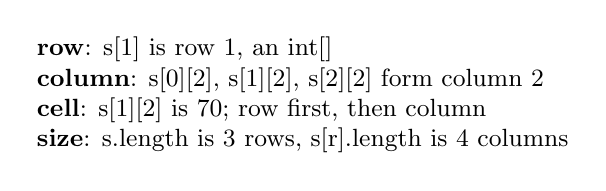
\begin{tikzpicture}
			\hGrid[id=g, name={s}, width=0.8, rowhot={1}, colhot={2}, hot={1/2}]{{72,85,90,64},{55,61,70,80},{90,88,93,99}}
			\node[font=\small, anchor=west, align=left] at (4.0,-0.25) {%
				\textbf{row}: \hCode{s[1]} is row 1, an \hCode{int[]}\\
				\textbf{column}: \hCode{s[0][2]}, \hCode{s[1][2]}, \hCode{s[2][2]} form column 2\\
				\textbf{cell}: \hCode{s[1][2]} is 70; row first, then column\\
				\textbf{size}: \hCode{s.length} is 3 rows, \hCode{s[r].length} is 4 columns};
		\end{tikzpicture}
	\end{center}

	\small $3 \times 4 = 12$ cells under one name. The rows are the students, the columns the quizzes.
\end{frame}
% ~~~~~~~~~~~~~~~~~~~~~~~~~~~~~~~~~~~~~~ A frm




% ~~~~~~~~~~~~~~~~~~~~~~~~~~~~~~~~~~~~~~ V
\hSection[Basics]{Creating and using a table}[\small Two indices, two loops]
% ~~~~~~~~~~~~~~~~~~~~~~~~~~~~~~~~~~~~~~ A




% ~~~~~~~~~~~~~~~~~~~~~~~~~~~~~~~~~~~~~~ V frm
\begin{frame}[t,fragile] \frametitle{Declaring and creating: two steps}


% +++++++++++++++++++++++++++++++++++++++ V lst
%: -Lst. two steps
\begin{lstlisting}[style=codesnippet, language=Java]
int[][] scores;              // 1. a variable that can refer to a table of ints
scores = new int[3][4];      // 2. the table itself: 3 rows, 4 columns, all 0

final int WEEKS = 4, DAYS = 7;
double[][] highs = new double[WEEKS][DAYS];   // both steps in one line
\end{lstlisting}
% +++++++++++++++++++++++++++++++++++++++ A lst


	\begin{center}
		\begin{tikzpicture}
			\node[font=\ttfamily\small] (t) at (0,0) {double[][]};
			\node[font=\ttfamily\small, right=0.7cm of t] (n) {highs};
			\node[font=\ttfamily\small, right=0.5cm of n] (e) {=};
			\node[font=\ttfamily\small, right=0.5cm of e] (v) {new double[WEEKS][DAYS]};
			\node[font=\scriptsize, below=0.3cm of t, align=center] {element type\\ and \hCode{[][]}};
			\node[font=\scriptsize, below=0.3cm of n, align=center] {name};
			\node[font=\scriptsize, below=0.3cm of v, align=center] {creates 4 rows of 7 elements;\\ the rows come first};
		\end{tikzpicture}
	\end{center}

	\begin{itemize}\small
		\item Two pairs of brackets: \hCode{double[][]} is read ``double array array'', an array whose elements are rows
		\item Always \hCode{[rows][columns]}; named constants say which number is which
	\end{itemize}
\end{frame}
% ~~~~~~~~~~~~~~~~~~~~~~~~~~~~~~~~~~~~~~ A frm




% ~~~~~~~~~~~~~~~~~~~~~~~~~~~~~~~~~~~~~~ V frm
\begin{frame}[t,fragile] \frametitle{A first table}
	\lstcoderightstep[0.66][basicstyle=\ttfamily\scriptsize]{codeoutput/FirstTable.java}{Java}{codeoutput/FirstTable.txt}

	\small \hQuestion{What does it print? Look at line 6.}
	\uncover<2->{Nobody wrote \hCode{t[1][0]}: it keeps its start value 0.}

	\footnotesize \uncover<2->{A list of rows \hCode{\{\{\dots\}, \{\dots\}\}} gives the values: \hCode{m.length} rows of \hCode{m[0].length} cells.}
\end{frame}
% ~~~~~~~~~~~~~~~~~~~~~~~~~~~~~~~~~~~~~~ A frm



\ifActivities % EXTRA activities V




% ~~~~~~~~~~~~~~~~~~~~~~~~~~~~~~~~~~~~~~ V frm
\begin{frame}[t,fragile] \frametitle{Quick check: create}
	\hCode{int[][] g = new int[2][5];}

	\begin{enumerate}
		\item What is \hCode{g.length}? \uncover<2->{\hEmph{2}, the rows}
		\item What is \hCode{g[0].length}? \uncover<2->{\hEmph{5}, the cells of row 0}
		\item Which is the last cell? \uncover<2->{\hCode{g[1][4]}}
		\item What is \hCode{g[1][4]} right now? \uncover<2->{\hEmph{0}, the start value}
		\item Make the table \hCode{\{\{1, 2\}, \{3, 4\}\}} in one line. \uncover<2->{\hCode{int[][] h = \{\{1, 2\}, \{3, 4\}\};}}
	\end{enumerate}
\end{frame}
% ~~~~~~~~~~~~~~~~~~~~~~~~~~~~~~~~~~~~~~ A frm



\fi % EXTRA activities A




% ~~~~~~~~~~~~~~~~~~~~~~~~~~~~~~~~~~~~~~ V frm
\begin{frame}[t,fragile] \frametitle{Visiting every cell: row by row}
	\begin{center}
		\begin{tikzpicture}
			\only<1>{\hGrid[id=t, name={t}, width=0.8, cur={0/0}]{{72,85,90},{55,61,70}}}
			\only<2>{\hGrid[id=t, name={t}, width=0.8, done={0/0}, cur={0/1}]{{72,85,90},{55,61,70}}}
			\only<3>{\hGrid[id=t, name={t}, width=0.8, done={0/0,0/1}, cur={0/2}]{{72,85,90},{55,61,70}}}
			\only<4>{\hGrid[id=t, name={t}, width=0.8, done={0/0,0/1,0/2}, cur={1/0}]{{72,85,90},{55,61,70}}}
			\only<5>{\hGrid[id=t, name={t}, width=0.8, done={0/0,0/1,0/2,1/0}, cur={1/1}]{{72,85,90},{55,61,70}}}
			\only<6>{\hGrid[id=t, name={t}, width=0.8, done={0/0,0/1,0/2,1/0,1/1}, cur={1/2}]{{72,85,90},{55,61,70}}}
			\only<7>{\hGrid[id=t, name={t}, width=0.8, done={0/0,0/1,0/2,1/0,1/1,1/2}]{{72,85,90},{55,61,70}}}
			\node[font=\ttfamily\small, anchor=west, colorTop!60!black] at (2.8,0.0) {%
				\only<1>{r = 0, c = 0}\only<2>{r = 0, c = 1}\only<3>{r = 0, c = 2}%
				\only<4>{r = 1, c = 0}\only<5>{r = 1, c = 1}\only<6>{r = 1, c = 2}%
				\only<7>{r == t.length: stop}};
		\end{tikzpicture}
	\end{center}


% +++++++++++++++++++++++++++++++++++++++ V lst
%: -Lst. row by row
\begin{lstlisting}[style=codesnippet, language=Java]
for (int r = 0; r < t.length; r++) {             // every row
    for (int c = 0; c < t[r].length; c++) {      // every column of row r
        System.out.print(t[r][c] + " ");
    }
    System.out.println();                        // row r is done
}
\end{lstlisting}
% +++++++++++++++++++++++++++++++++++++++ A lst


	\small \hCode{t.length}: the number of rows. \hCode{t[r].length}: the length of row \hCode{r}.
	The inner loop runs completely for every \hCode{r}: the nested loops of week 5.
\end{frame}
% ~~~~~~~~~~~~~~~~~~~~~~~~~~~~~~~~~~~~~~ A frm




% ~~~~~~~~~~~~~~~~~~~~~~~~~~~~~~~~~~~~~~ V frm
\begin{frame}[t,fragile] \frametitle{The enhanced for loop on a table}


% +++++++++++++++++++++++++++++++++++++++ V lst
%: -Lst. enhanced for on a table
\begin{lstlisting}[style=codesnippet, language=Java]
for (int[] row : t) { for (int x : row) { ... } }   // for each row, each x in it
\end{lstlisting}
% +++++++++++++++++++++++++++++++++++++++ A lst


	\footnotesize The outer variable is a whole row, an \hCode{int[]}; the inner loop is the enhanced for of week 7 on that row.

	\lstcoderightstep[0.66][basicstyle=\ttfamily\scriptsize, firstline=3, lastline=10, firstnumber=3]{codeoutput/ForEachTable.java}{Java}{codeoutput/ForEachTable.txt}

	\footnotesize \uncover<2->{Read only, and no indices: to write cells, or to know \hCode{r} and \hCode{c}, use the index loops.}
\end{frame}
% ~~~~~~~~~~~~~~~~~~~~~~~~~~~~~~~~~~~~~~ A frm




% ~~~~~~~~~~~~~~~~~~~~~~~~~~~~~~~~~~~~~~ V frm
\begin{frame}[t,fragile] \frametitle{Rows and columns mixed up}
	\footnotesize \hQuestion{The table has 2 rows and 3 columns. What goes wrong?}

	\lstcodedownstep[basicstyle=\ttfamily\scriptsize, firstline=3, lastline=9, firstnumber=3][basicstyle=\ttfamily\fontsize{6.4}{7.6}\selectfont]{codeoutput/SwappedIndex.java}{Java}{codeoutput/SwappedIndex.txt}

	\begin{itemize}\footnotesize
		\item<3-> The outer loop counts to 3, but there are only 2 rows: \hCode{t[2]} does not exist.
			  The program stops with the out-of-bounds error of week 7, at line 6.
		\item<3-> On a square table this bug hides. Rule: \hCode{r} goes with \hCode{t.length},
			  \hCode{c} with \hCode{t[r].length}.
	\end{itemize}
\end{frame}
% ~~~~~~~~~~~~~~~~~~~~~~~~~~~~~~~~~~~~~~ A frm




% ~~~~~~~~~~~~~~~~~~~~~~~~~~~~~~~~~~~~~~ V frm
\begin{frame}[t,fragile] \frametitle{Two errors the compiler finds}
	\lstoutput[basicstyle=\ttfamily\scriptsize]{codeoutput/CommaIndex.txt}

	\footnotesize \hCode{t[1, 2]} is not Java: one pair of brackets per index, \hCode{t[1][2]}.

	\vspace{0.5em}
	\lstoutput[basicstyle=\ttfamily\scriptsize]{codeoutput/NoRowCount.txt}

	\footnotesize The number of rows is required. \hCode{new int[3][]} is allowed (the rows come later);
	\hCode{new int[][3]} is not.
\end{frame}
% ~~~~~~~~~~~~~~~~~~~~~~~~~~~~~~~~~~~~~~ A frm




% ~~~~~~~~~~~~~~~~~~~~~~~~~~~~~~~~~~~~~~ V frm
\begin{frame}[t,fragile] \frametitle{Printing a table}
	\lstcoderightstep[0.66][basicstyle=\ttfamily\scriptsize]{codeoutput/PrintTable.java}{Java}{codeoutput/PrintTable.txt}

	\footnotesize \uncover<2->{\hCode{println} and \hCode{Arrays.toString} show only arrows; \hCode{Arrays.deepToString} shows the cells.
	\hCode{printf("\%4d", \dots)} (week 3) makes straight columns.}
\end{frame}
% ~~~~~~~~~~~~~~~~~~~~~~~~~~~~~~~~~~~~~~ A frm




% ~~~~~~~~~~~~~~~~~~~~~~~~~~~~~~~~~~~~~~ V frm
\begin{frame}[t,fragile] \frametitle{A table is an array of rows}
	\begin{center}
		\begin{tikzpicture}
			\node[hvar] (v) at (0,0.25) {};
			\node[font=\ttfamily\small, left=2pt of v] {t};
			\hArray[id=o, at={(1.2,0)}, width=0.6, font=\ttfamily\scriptsize]{\phantom{0},\phantom{0}}
			\hArray[id=a, at={(3.6,0.75)}, width=0.6]{1,2,3}
			\hArray[id=b, at={(3.6,-0.55)}, width=0.6]{4,5,6}
			\draw[href] (v.center) -- (o-0.west);
			\draw[href] (o-0.center) -- (a-0.west);
			\draw[href] (o-1.center) -- (b-0.west);
			\node[font=\small, anchor=west] at (5.7,1.0) {\hCode{t[0]}, a row: an \hCode{int[]}};
			\node[font=\small, anchor=west] at (5.7,-0.3) {\hCode{t[1]}};
		\end{tikzpicture}
	\end{center}

	\lstcoderightstep[0.66][basicstyle=\ttfamily\scriptsize]{codeoutput/RowsAreArrays.java}{Java}{codeoutput/RowsAreArrays.txt}

	\footnotesize \uncover<2->{\hCode{row} is a second arrow to row 1 (an alias, week 7). Line 7 gives the table a new, shorter row 0.}
\end{frame}
% ~~~~~~~~~~~~~~~~~~~~~~~~~~~~~~~~~~~~~~ A frm




% ~~~~~~~~~~~~~~~~~~~~~~~~~~~~~~~~~~~~~~ V frm
\begin{frame}[t,fragile] \frametitle{Rows of different lengths}
	\lstcoderightstep[0.66][basicstyle=\ttfamily\scriptsize]{codeoutput/Ragged.java}{Java}{codeoutput/Ragged.txt}

	\footnotesize \hCode{new int[4][]} makes 4 rows that do not exist yet; line 5 creates each one.
	Such a \hDefined{ragged} table is why loops use \hCode{t[r].length}, not \hCode{t[0].length}.
\end{frame}
% ~~~~~~~~~~~~~~~~~~~~~~~~~~~~~~~~~~~~~~ A frm



\ifActivities % EXTRA activities V




% ~~~~~~~~~~~~~~~~~~~~~~~~~~~~~~~~~~~~~~ V frm
\begin{frame}[t,fragile] \frametitle{On paper: draw the arrows}
	Draw the variables, the arrows and the rows after each line. Then answer.


% +++++++++++++++++++++++++++++++++++++++ V lst
%: -Lst. draw it
\begin{lstlisting}[style=codesnippet, language=Java]
int[][] a = {{1, 2}, {3, 4}};
int[][] b = a;
int[][] c = java.util.Arrays.copyOf(a, a.length);
c[0][0] = 9;
c[1] = new int[] {5, 6};
\end{lstlisting}
% +++++++++++++++++++++++++++++++++++++++ A lst


	\begin{enumerate}\small
		\item What is \hCode{a[0][0]}? \uncover<2->{\hEmph{9}: \hCode{c} is a new array of arrows, but to the \emph{same} rows}
		\item What is \hCode{a[1][0]}? \uncover<2->{\hEmph{3}: \hCode{c[1]} now points to a new row; row 1 of \hCode{a} is unchanged}
		\item How many rows (\hCode{int[]}) are there? \uncover<2->{\hEmph{3}: the two rows of \hCode{a}, and \hCode{\{5, 6\}}}
	\end{enumerate}
	\uncover<2->{\small Copying a table copies only the arrows to its rows. To copy the cells, copy every row.}
\end{frame}
% ~~~~~~~~~~~~~~~~~~~~~~~~~~~~~~~~~~~~~~ A frm



\fi % EXTRA activities A




% ~~~~~~~~~~~~~~~~~~~~~~~~~~~~~~~~~~~~~~ V
\hSection[Algos]{Common table algorithms}[\small The patterns of week 7, by row and by column]
% ~~~~~~~~~~~~~~~~~~~~~~~~~~~~~~~~~~~~~~ A




% ~~~~~~~~~~~~~~~~~~~~~~~~~~~~~~~~~~~~~~ V frm
\begin{frame}[t,fragile] \frametitle{A catalogue of table patterns}


% +++++++++++++++++++++++++++++++++++++++ V tbl
%: -Tbl. table patterns
\begin{table}
		\footnotesize
		\begin{tabular}{@{}L{0.12\textwidth}L{0.19\textwidth}L{0.16\textwidth}L{0.29\textwidth}L{0.12\textwidth}@{}}
			\toprule
			\textbf{Pattern} & \textbf{Question} & \textbf{Loops} & \textbf{At cell $(r, c)$} & \textbf{Result} \\
			\midrule
			Row total    & each row's sum?       & $r$ outside, $c$ inside & $s \gets s + t[r][c]$                 & one per row \\
			Column total & each column's sum?    & $c$ outside, $r$ inside & $s \gets s + t[r][c]$                 & one per column \\
			Largest      & the largest cell?     & $r$, $c$                & if $t[r][c] > t[b_{r}][b_{c}]$: keep $r, c$ & $b_{r}$, $b_{c}$ \\
			Search       & where is $x$?         & both stop early         & if $t[r][c] = x$: keep $r, c$         & $r, c$ or $-1$ \\
			Count        & how many match?       & $r$, $c$                & if match: $n \gets n + 1$             & $n$ \\
			Neighbors    & the cells around      & none                    & check the edge first                  & up to 4 cells \\
			Diagonal     & $t[i][i]$             & one loop, $i$           & square tables only                    & $n$ cells \\
			\bottomrule
		\end{tabular}
\end{table}%
% +++++++++++++++++++++++++++++++++++++++ A tbl


	\vspace{0.3em}
	\small Every pattern of week 7 works on a table. First decide: per row, per column, or over all cells?
\end{frame}
% ~~~~~~~~~~~~~~~~~~~~~~~~~~~~~~~~~~~~~~ A frm




% ~~~~~~~~~~~~~~~~~~~~~~~~~~~~~~~~~~~~~~ V frm
\begin{frame}[t,fragile] \frametitle{Row totals and column totals}
	\lstcoderightstep[0.66][basicstyle=\ttfamily\scriptsize, firstline=3, lastline=19, firstnumber=3]{codeoutput/RowColTotals.java}{Java}{codeoutput/RowColTotals.txt}

	\footnotesize Column totals: the column loop is outside, the row loop inside.
	\hCode{s[0].length} is the number of columns only in a rectangular table.
\end{frame}
% ~~~~~~~~~~~~~~~~~~~~~~~~~~~~~~~~~~~~~~ A frm




% ~~~~~~~~~~~~~~~~~~~~~~~~~~~~~~~~~~~~~~ V frm
\begin{frame}[t,fragile] \frametitle{The largest cell}
	\lstcoderightstep[0.66][basicstyle=\ttfamily\scriptsize, firstline=3, lastline=17, firstnumber=3]{codeoutput/LargestCell.java}{Java}{codeoutput/LargestCell.txt}

	\footnotesize Keep the row \emph{and} the column of the best so far; start with cell $(0, 0)$.
\end{frame}
% ~~~~~~~~~~~~~~~~~~~~~~~~~~~~~~~~~~~~~~ A frm



\ifActivities % EXTRA activities V




% ~~~~~~~~~~~~~~~~~~~~~~~~~~~~~~~~~~~~~~ V frm
\begin{frame}[t,fragile] \frametitle{On paper: trace the largest-cell loops}
	\hCode{t = \{\{4, 9, 2\}, \{9, 1, 7\}\}}; fill one row per step, then click.


% +++++++++++++++++++++++++++++++++++++++ V tbl
%: -Tbl. trace
\begin{table}
		\small
		\begin{tabular}{@{}cccccc@{}}
			\toprule
			\hCode{r} & \hCode{c} & \hCode{t[r][c]} & \hCode{t[r][c] > t[br][bc]}? & \hCode{br} & \hCode{bc} \\
			\midrule
			start & --  & --  & --                                  & 0                          & 0 \\
			0     & 0   & 4   & \leavevmode\uncover<2->{no}         & \leavevmode\uncover<2->{0} & \leavevmode\uncover<2->{0} \\
			0     & 1   & 9   & \leavevmode\uncover<2->{yes}        & \leavevmode\uncover<2->{0} & \leavevmode\uncover<2->{1} \\
			0     & 2   & 2   & \leavevmode\uncover<2->{no}         & \leavevmode\uncover<2->{0} & \leavevmode\uncover<2->{1} \\
			1     & 0   & 9   & \leavevmode\uncover<2->{no, equal}  & \leavevmode\uncover<2->{0} & \leavevmode\uncover<2->{1} \\
			1     & 1   & 1   & \leavevmode\uncover<2->{no}         & \leavevmode\uncover<2->{0} & \leavevmode\uncover<2->{1} \\
			1     & 2   & 7   & \leavevmode\uncover<2->{no}         & \leavevmode\uncover<2->{0} & \leavevmode\uncover<2->{1} \\
			\bottomrule
		\end{tabular}
\end{table}%
% +++++++++++++++++++++++++++++++++++++++ A tbl


	\vspace{0.3em}
	\small \uncover<2->{Cell $(0, 1)$ wins the tie: row by row, the first 9 is met first.}
\end{frame}
% ~~~~~~~~~~~~~~~~~~~~~~~~~~~~~~~~~~~~~~ A frm



\fi % EXTRA activities A




% ~~~~~~~~~~~~~~~~~~~~~~~~~~~~~~~~~~~~~~ V frm
\begin{frame}[t,fragile] \frametitle{Searching a table}
	\lstcoderightstep[0.66][basicstyle=\ttfamily\scriptsize, firstline=3, lastline=17, firstnumber=3]{codeoutput/FindCell.java}{Java}{codeoutput/FindCell.txt}

	\footnotesize \hCode{fr == -1} is in both loop conditions, so both loops stop at the first match.
	$-1$ means ``not found'': it is never an index (week 7).
\end{frame}
% ~~~~~~~~~~~~~~~~~~~~~~~~~~~~~~~~~~~~~~ A frm




% ~~~~~~~~~~~~~~~~~~~~~~~~~~~~~~~~~~~~~~ V frm
\begin{frame}[t,fragile] \frametitle{The neighbors of a cell}
	\begin{columns}[T]
		\begin{column}{0.30\textwidth}
			\begin{center}
				\begin{tikzpicture}
					\hGrid[id=h, name={h}, width=0.6, hot={0/1}, cur={0/0,0/2,1/1}]{{1,2,3},{4,5,6},{7,8,9}}
				\end{tikzpicture}
			\end{center}
			\footnotesize Cell $(0, 1)$ is on the top edge: it has no ``up'' neighbor.
		\end{column}
		\begin{column}{0.68\textwidth}
			\lstcode[basicstyle=\ttfamily\scriptsize, firstline=6, lastline=14, firstnumber=6]{codeoutput/Neighbors.java}{Java}
			\uncover<2->{\lstoutput[basicstyle=\ttfamily\scriptsize]{codeoutput/Neighbors.txt}}
		\end{column}
	\end{columns}

	\vspace{0.3em}
	\footnotesize Up, down, left, right: $(r - 1, c)$, $(r + 1, c)$, $(r, c - 1)$, $(r, c + 1)$.
	Check the edge \emph{before} reading the cell, or the index is out of bounds.
\end{frame}
% ~~~~~~~~~~~~~~~~~~~~~~~~~~~~~~~~~~~~~~ A frm



\ifExtraAlgos % EXTRA algorithms V




% ~~~~~~~~~~~~~~~~~~~~~~~~~~~~~~~~~~~~~~ V frm
\begin{frame}[t,fragile] \frametitle{The diagonals of a square board}
	\begin{columns}[T]
		\begin{column}{0.66\textwidth}
			\lstcode[basicstyle=\ttfamily\scriptsize, firstline=3, lastline=13, firstnumber=3]{codeoutput/Diagonals.java}{Java}
		\end{column}
		\begin{column}{0.32\textwidth}
			\begin{center}
				\begin{tikzpicture}
					\hGrid[id=b, name={b}, width=0.6, hot={0/0,1/1,2/2}]{{X,O,X},{O,X,O},{O,\textvisiblespace,X}}
				\end{tikzpicture}
			\end{center}
			\uncover<2->{\lstoutput[basicstyle=\ttfamily\scriptsize]{codeoutput/Diagonals.txt}}
		\end{column}
	\end{columns}

	\footnotesize \hCode{b[i][i]} is the diagonal from the top left; \hCode{b[i][n - 1 - i]} the other one,
	with the mirror index of week 7. One loop is enough.
\end{frame}
% ~~~~~~~~~~~~~~~~~~~~~~~~~~~~~~~~~~~~~~ A frm



\fi % EXTRA algorithms A




% ~~~~~~~~~~~~~~~~~~~~~~~~~~~~~~~~~~~~~~ V
\hSection[Methods]{Tables and methods}[\small A table parameter is an arrow, as in week 7]
% ~~~~~~~~~~~~~~~~~~~~~~~~~~~~~~~~~~~~~~ A




% ~~~~~~~~~~~~~~~~~~~~~~~~~~~~~~~~~~~~~~ V frm
\begin{frame}[t,fragile] \frametitle{Methods that take a table}
	\lstcode[basicstyle=\ttfamily\scriptsize, firstline=3, lastline=20, firstnumber=3]{codeoutput/TableMethods.java}{Java}

	\footnotesize \hQuestion{Which method changes the caller's table?}
	\uncover<2->{Neither: both only read \hCode{t}. Writing \hCode{t[r][c]} would change the caller's table.}
\end{frame}
% ~~~~~~~~~~~~~~~~~~~~~~~~~~~~~~~~~~~~~~ A frm




% ~~~~~~~~~~~~~~~~~~~~~~~~~~~~~~~~~~~~~~ V frm
\begin{frame}[t,fragile] \frametitle{Calling them}
	\lstcoderightstep[0.66][basicstyle=\ttfamily\scriptsize, firstline=21, lastline=25, firstnumber=21]{codeoutput/TableMethods.java}{Java}{codeoutput/TableMethods.txt}

	\begin{itemize}\small
		\item \hCode{rowTotals} returns an \hCode{int[]}: one number for every row
		\item \hCode{transpose} returns a new \hCode{int[][]}: row \hCode{r} becomes column \hCode{r},
			  so a $2 \times 4$ table becomes $4 \times 2$
		\item Both work for any number of rows and columns; nothing is fixed to 2 or 4
	\end{itemize}
\end{frame}
% ~~~~~~~~~~~~~~~~~~~~~~~~~~~~~~~~~~~~~~ A frm



\ifEclipseLab % EXTRA Eclipse and lab V




% ~~~~~~~~~~~~~~~~~~~~~~~~~~~~~~~~~~~~~~ V frm
\begin{frame}[t,fragile] \frametitle{In Eclipse: watch a table in the debugger}
	\begin{enumerate}\small
		\item Put a breakpoint on a line inside the inner loop of \hCode{RowColTotals}
		\item \menu{Run > Debug As > Java Application}; the keys are the ones of week 7
		\item In the \menu{Variables} view, open \hCode{s}: one row per entry, \hCode{[0]}, \hCode{[1]}, \hCode{[2]};
			  open a row to see its cells
		\item Step with \keys{F6} and watch \hCode{r}, \hCode{c} and \hCode{total}: the inner loop
			  runs to the end before \hCode{r} changes
		\item In the \menu{Expressions} view, add \hCode{s[r][c]}: the current cell, at every step
	\end{enumerate}

	\vspace{0.5em}
	\small \hRemark{Try}: break inside the column-total loops and see \hCode{r} change faster than \hCode{c}.
\end{frame}
% ~~~~~~~~~~~~~~~~~~~~~~~~~~~~~~~~~~~~~~ A frm



\fi % EXTRA Eclipse and lab A



\ifActivities % EXTRA activities V




% ~~~~~~~~~~~~~~~~~~~~~~~~~~~~~~~~~~~~~~ V frm
\begin{frame}[t,fragile] \frametitle{Quick check: methods}


% +++++++++++++++++++++++++++++++++++++++ V lst
%: -Lst. methods quiz
\begin{lstlisting}[style=codesnippet, language=Java]
static void newRow(int[][] t, int r) { t[r] = new int[t[r].length]; }
static void newTable(int[][] t) { t = new int[2][2]; }
int[][] x = {{1, 2}, {3, 4}};   newTable(x);   newRow(x, 0);
\end{lstlisting}
% +++++++++++++++++++++++++++++++++++++++ A lst


	\begin{enumerate}
		\item After \hCode{newTable(x)}, what is \hCode{x[0][0]}? \uncover<2->{\hEmph{1}: only the parameter's arrow moved}
		\item After \hCode{newRow(x, 0)}, what is \hCode{x[0][0]}? \uncover<2->{\hEmph{0}: \hCode{t[r]} is a cell of the
			  caller's array of rows, so the caller gets the new row}
		\item Write the header of a method that returns the column totals.
			  \uncover<2->{\hCode{static int[] columnTotals(int[][] t)}}
	\end{enumerate}
\end{frame}
% ~~~~~~~~~~~~~~~~~~~~~~~~~~~~~~~~~~~~~~ A frm



\fi % EXTRA activities A




% ~~~~~~~~~~~~~~~~~~~~~~~~~~~~~~~~~~~~~~ V
\hSection[ND]{More dimensions}[\small One more index, one more loop]
% ~~~~~~~~~~~~~~~~~~~~~~~~~~~~~~~~~~~~~~ A




% ~~~~~~~~~~~~~~~~~~~~~~~~~~~~~~~~~~~~~~ V frm
\begin{frame}[t,fragile] \frametitle{Three dimensions: an array of tables}
	\begin{center}
		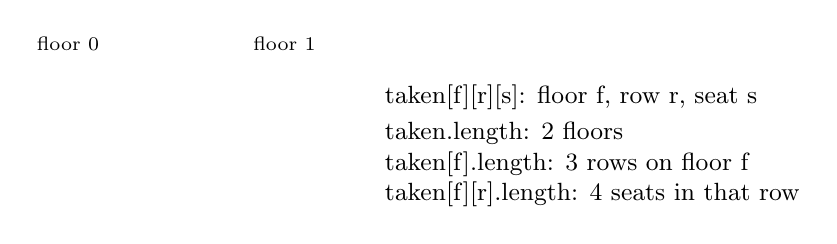
\begin{tikzpicture}
			\hGrid[id=f0, at={(0,0)}, width=0.55, hot={1/2}]{{\phantom{0},,,},{,,,},{,,,\phantom{0}}}
			\node[font=\scriptsize] at (1.1,1.05) {floor 0};
			\hGrid[id=f1, at={(2.75,0)}, width=0.55, hot={0/0,2/3}]{{\phantom{0},,,},{,,,},{,,,\phantom{0}}}
			\node[font=\scriptsize] at (3.85,1.05) {floor 1};
			\node[font=\small, anchor=west, align=left] at (5.0,-0.25) {%
				\hCode{taken[f][r][s]}: floor \hCode{f}, row \hCode{r}, seat \hCode{s}\\[2pt]
				\hCode{taken.length}: 2 floors\\
				\hCode{taken[f].length}: 3 rows on floor \hCode{f}\\
				\hCode{taken[f][r].length}: 4 seats in that row};
		\end{tikzpicture}
	\end{center}

	\begin{itemize}\small
		\item \hCode{new boolean[2][3][4]}: 2 tables of 3 rows of 4 seats, $2 \cdot 3 \cdot 4 = 24$ cells, all \hCode{false}
		\item A 3D array is an array of tables, just as a table is an array of rows
	\end{itemize}
\end{frame}
% ~~~~~~~~~~~~~~~~~~~~~~~~~~~~~~~~~~~~~~ A frm




% ~~~~~~~~~~~~~~~~~~~~~~~~~~~~~~~~~~~~~~ V frm
\begin{frame}[t,fragile] \frametitle{Three indices, three loops}
	\lstcoderightstep[0.66][basicstyle=\ttfamily\scriptsize]{codeoutput/ThreeD.java}{Java}{codeoutput/ThreeD.txt}

	\footnotesize Each loop takes its bound from the level above it: floors, then rows of floor \hCode{f}, then seats of that row.
\end{frame}
% ~~~~~~~~~~~~~~~~~~~~~~~~~~~~~~~~~~~~~~ A frm




% ~~~~~~~~~~~~~~~~~~~~~~~~~~~~~~~~~~~~~~ V frm
\begin{frame}[t,fragile] \frametitle{N dimensions}


% +++++++++++++++++++++++++++++++++++++++ V tbl
%: -Tbl. dimensions
\begin{table}
		\small
		\begin{tabular}{@{}L{0.07\textwidth}L{0.20\textwidth}L{0.16\textwidth}L{0.14\textwidth}L{0.25\textwidth}@{}}
			\toprule
			\textbf{N} & \textbf{Type} & \textbf{One element} & \textbf{Loops} & \textbf{Example} \\
			\midrule
			1 & \hCode{int[]}       & \hCode{a[i]}       & 1        & a list of scores \\
			2 & \hCode{int[][]}     & \hCode{t[r][c]}    & 2        & students $\times$ quizzes \\
			3 & \hCode{int[][][]}   & \hCode{d[f][r][s]} & 3        & floors $\times$ rows $\times$ seats \\
			N & N pairs of \hCode{[]} & N indices        & N nested & rare beyond 3 \\
			\bottomrule
		\end{tabular}
\end{table}%
% +++++++++++++++++++++++++++++++++++++++ A tbl


	\vspace{0.5em}
	\begin{itemize}\small
		\item Every \hCode{[]} adds one index, and usually one loop
		\item An N-dimensional array is an array of (N $-$ 1)-dimensional arrays
		\item The number of cells is the product of the lengths: it grows fast
	\end{itemize}
\end{frame}
% ~~~~~~~~~~~~~~~~~~~~~~~~~~~~~~~~~~~~~~ A frm




% ~~~~~~~~~~~~~~~~~~~~~~~~~~~~~~~~~~~~~~ V
\hSection[End]{Summary}
% ~~~~~~~~~~~~~~~~~~~~~~~~~~~~~~~~~~~~~~ A




% ~~~~~~~~~~~~~~~~~~~~~~~~~~~~~~~~~~~~~~ V frm
\begin{frame}[t,fragile] \frametitle{Cheat sheet}


% +++++++++++++++++++++++++++++++++++++++ V lst
%: -Lst. cheat sheet
\begin{lstlisting}[style=codesnippet, language=Java, basicstyle=\ttfamily\scriptsize]
int[][] t = new int[3][4];               // 3 rows, 4 columns, all 0
int[][] m = {{1, 2, 3}, {4, 5, 6}};      // a list of rows
t[1][2] = 7;   int x = m[0][1];          // write, read: [row][column]
int rows = t.length;                     // the number of rows
int cols = t[0].length;                  // the length of row 0
for (int r = 0; r < t.length; r++) {             // row by row
    for (int c = 0; c < t[r].length; c++) { ... t[r][c] ... }
}
for (int[] row : t) { for (int v : row) { ... } }   // read only
int[] row1 = t[1];                       // a row is an int[]
int[][] tri = new int[4][];              // rows later: a ragged table
System.out.println(Arrays.deepToString(t));         // every cell
static int[][] transpose(int[][] t) {...}           // a table in, a table out
\end{lstlisting}
% +++++++++++++++++++++++++++++++++++++++ A lst


	\footnotesize Patterns: per row, per column, over all cells; neighbors after an edge check; diagonals of square tables.
\end{frame}
% ~~~~~~~~~~~~~~~~~~~~~~~~~~~~~~~~~~~~~~ A frm




% ~~~~~~~~~~~~~~~~~~~~~~~~~~~~~~~~~~~~~~ V frm
\begin{frame}[t,fragile] \frametitle{Exercises}
	\begin{enumerate}\small
		\item Fill a $10 \times 10$ multiplication table and print it in straight columns with \hCode{printf}.
		\item For the quiz table, print the average of every quiz (every column).
		\item Write \hCode{static boolean isSymmetric(int[][] t)}: is \hCode{t[r][c] == t[c][r]} for every cell of a square table?
		\item Count the cells that are larger than all of their (up to 4) neighbors.
		\item A theater has rows of 8, 10 and 12 seats. Store it as a ragged \hCode{boolean[][]} and count the free seats.
		\item For the three-dimensional \hCode{taken}, print the number of taken seats on every floor.
	\end{enumerate}
\end{frame}
% ~~~~~~~~~~~~~~~~~~~~~~~~~~~~~~~~~~~~~~ A frm




% ~~~~~~~~~~~~~~~~~~~~~~~~~~~~~~~~~~~~~~ V frm
\begin{frame}[t,fragile] \frametitle{Where tables come back}


% +++++++++++++++++++++++++++++++++++++++ V tbl
%: -Tbl. next weeks
\begin{table}
		\small
		\begin{tabular}{@{}L{0.12\textwidth}L{0.24\textwidth}L{0.56\textwidth}@{}}
			\toprule
			\textbf{When} & \textbf{Topic} & \textbf{Tables there} \\
			\midrule
			week 9  & String              & a \hCode{String[]} of lines is a table of characters: \hCode{lines[r].charAt(c)} \\
			week 10 & Input/Output        & read a table from a file, one row per line \\
			week 11 & Exceptions, testing & today's out-of-bounds errors are exceptions; tests compare tables \\
			week 12 & Recursion           & walk a grid or a maze cell by cell \\
			CIS112  & Data structures     & a graph as a table: \hCode{adj[u][v]} says whether \hCode{u} and \hCode{v} are connected \\
			\bottomrule
		\end{tabular}
\end{table}%
% +++++++++++++++++++++++++++++++++++++++ A tbl


	\vspace{0.3em}
	\small Reading: bjlo2, Chapter 6, two-dimensional arrays. Decks of this topic: \hCode{arrayND-0-concepts} \dots\ \hCode{arrayND-5-examples}.
\end{frame}
% ~~~~~~~~~~~~~~~~~~~~~~~~~~~~~~~~~~~~~~ A frm




% ~~~~~~~~~~~~~~~~~~~~~~~~~~~~~~~~~~~~~~ V frm
\begin{frame}[t,fragile] \frametitle{References}
	\small The Java Tutorials, Arrays \cite{TheJavaTutorialsArray}; Big Java \cite{horstmann2016big}.

	\vspace{1em}
	\setbeamertemplate{bibliography item}[text]
	\bibliographystyle{IEEEtran}
	\tiny\bibliography{../../hblib/hblibDataStructures}
\end{frame}
% ~~~~~~~~~~~~~~~~~~~~~~~~~~~~~~~~~~~~~~ A frm




% ~~~~~~~~~~~~~~~~~~~~~~~~~~~~~~~~~~~~~~ V frm
\begin{frame}[t,fragile]
	\begin{center}
		\vspace{4cm}
		\hRemark{\Huge Questions?}
	\end{center}
\end{frame}
% ~~~~~~~~~~~~~~~~~~~~~~~~~~~~~~~~~~~~~~ A frm



\end{document}
